\bfseries

\title[PTTC School and Workshop in Houston 2010]{Introduction to \\ \textsc{Madagascar} Software Package}

\author[S. Fomel] % (optional)
{Sergey~Fomel}

\institute[Madagascar School and Hands-On Workshop] % (optional)
{
  Bureau of Economic Geology \\
%  Jackson School of Geosciences \\
  The University of Texas at Austin
}

\date{July 23, 2010}

\setbeamercolor{quotecol}{fg=black,bg=white}

\newcommand{\quotebox}[3]{
  \begin{beamercolorbox}[wd=\textwidth,center]{quotecol}
    \begin{quote}
      #1 
      \color{blue}{\emph{#2}, #3}
    \end{quote}
    \end{beamercolorbox}
}

\begin{frame}
  \MadLogo
  \PTTCLogo
  \titlepage
\end{frame}

\begin{frame}
\MadLogo
\frametitle{Agenda for Friday, July 23}
\noindent\begin{tabular}{|rcl|l|l|} 
\hline 
9:00 & -- & 10:30 & Sergey Fomel & {\color{blue}{Introduction}} \\
\hline
10:45 & -- & 12:15 & Paul Sava & Seismic finite-difference \\
          &      &           &                & modeling and migration \\
\hline 12:15 & -- & 1:15 & \multicolumn{2}{|l|}{Lunch} \\
\hline 1:15 & -- & 2:45 & Jim Jennings & Workflows in SCons \\
                  &      &         &                      & and
                  automatic testing \\
\hline 3:00 & -- & 4:30 & \multicolumn{2}{|l|}{Discussion} \\
\hline 5:30 & -- & 8:00 & \multicolumn{2}{|l|}{Dinner and
  \textsc{Madagascar}  1.0 celebration} \\
\hline 
\end{tabular}
\end{frame}

\begin{frame}
\MadLogo
\frametitle{Agenda for Saturday, July 24}
\noindent\begin{tabular}{|rcl|l|l|} 
\hline 
9:00 & -- & 9:30 & Tariq Alkhalifah & Learning \\
        &      &         &                           & \textsc{Madagascar} \\
\hline 
9:00 & -- & 9:30 & Jeff Godwin & Programming with \\
        &      &         &                    & \textsc{Madagascar} \\
\hline
10:45 & -- & 11:15 & Joe Dellinger & Vplot graphics \\
\hline
11:15 & -- & 11:15 & Vladimir Bashkardin & Plotting and HPC \\
\hline 12:15 & -- & 1:15 & \multicolumn{2}{|l|}{Lunch} \\
\hline 1:15 & -- & 2:45 & Yang Liu & Seismic field data \\
                   &      &         &               & processing \\
\hline 3:00 & -- & 4:30 & \multicolumn{2}{|l|}{Discussion} \\
\hline 
\end{tabular}
\end{frame}

\section{History of Madagascar}

\begin{frame}
  \MadLogo
  \frametitle{Outline}
  \tableofcontents[pausesections]
\end{frame}

\begin{frame}<beamer>
  \MadLogo
  \frametitle{Outline}
  \tableofcontents[currentsection]
\end{frame}

\begin{frame}
\begin{minipage}{0.4\textwidth}
\quotebox{Black Magic in \\ Geophysical \\ Prospecting}{\\ L. W. Blau}{1936}
\end{minipage} \hfill
\begin{minipage}{0.5\textwidth}
\begin{center}
  
\includegraphics[height=\textheight]{Fig/magic}
\end{center}
\end{minipage}
\end{frame}

\begin{frame}
\frametitle{Black Magic in Computational Science}

\quotebox{ 
Within the world of science, computation is now rightly seen as a
third vertex of a triangle complementing experiment and
theory. However, as it is now often practiced, one can make a good
case that computing is the {\color{blue}{last refuge of the scientific scoundrel}} [...] 
Where else in science can one get away with publishing observations
that are claimed to prove a theory or illustrate the success of a
technique without having to give a careful description of the methods
used, in sufficient detail that others can attempt to repeat the
experiment?}{Randall LeVeque}{ICM, 2006}

\end{frame}

\begin{frame}
\MadLogo
\frametitle{(Hale, 1984)}
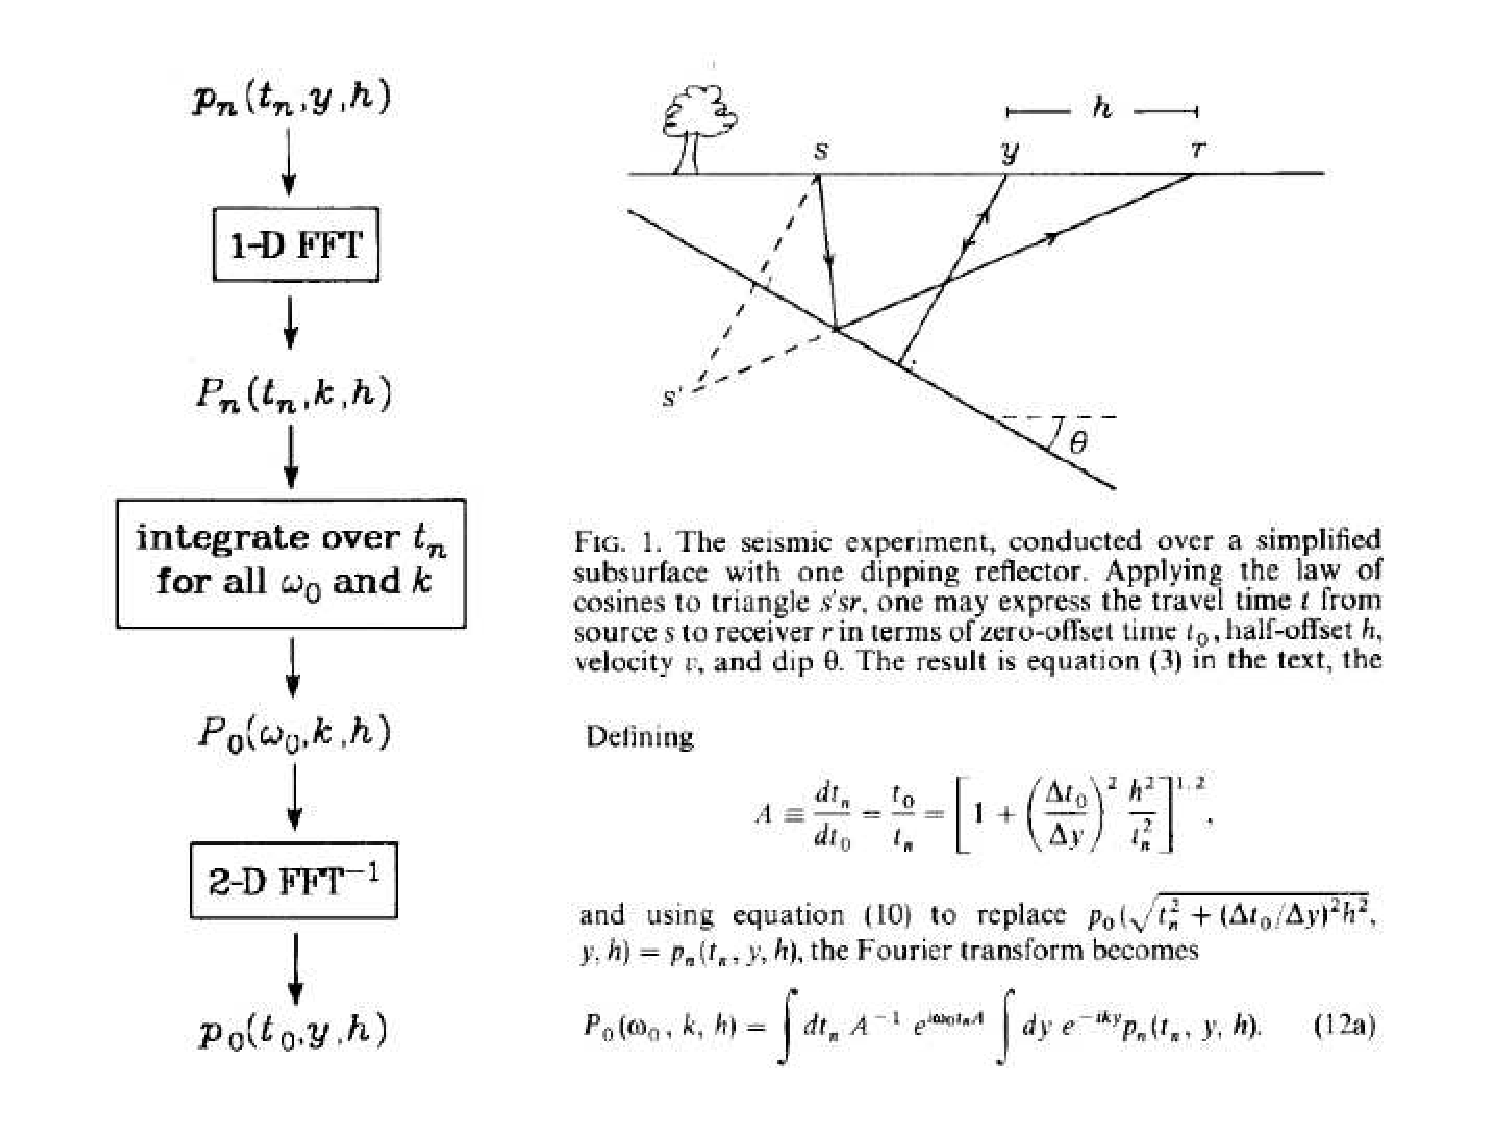
\includegraphics[height=0.8\textheight]{Fig/Hale1}
\end{frame}

\begin{frame}
\MadLogo
\frametitle{(Hale, 1984)}
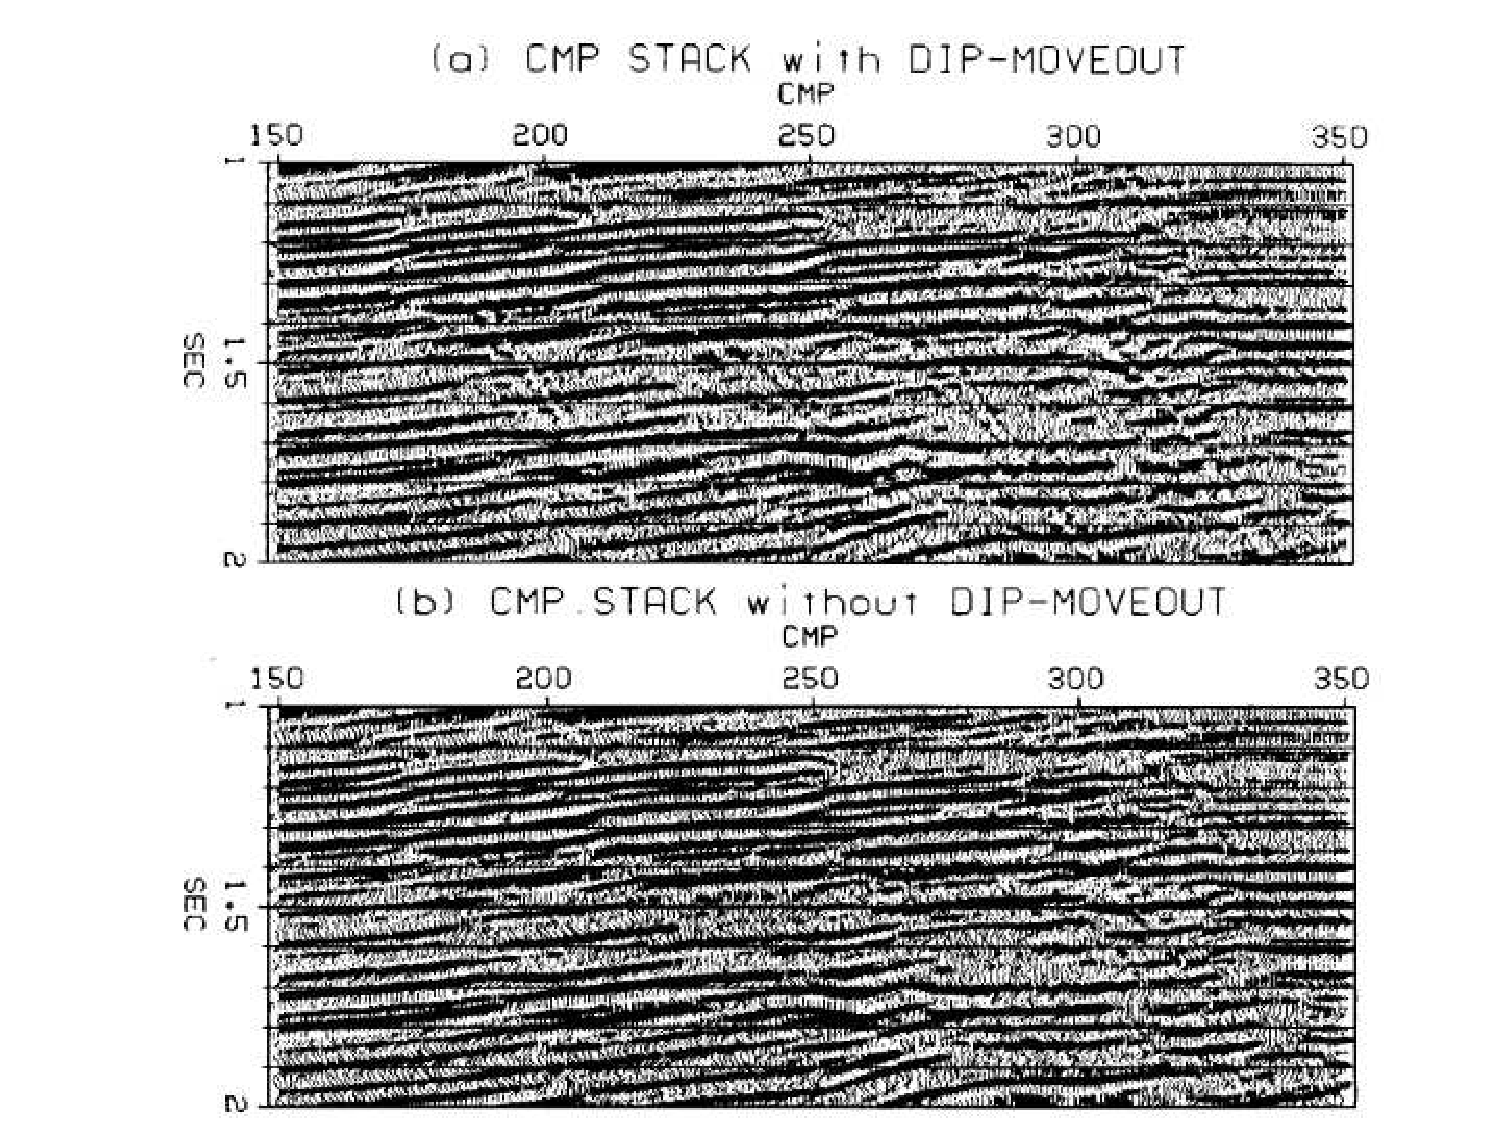
\includegraphics[height=0.8\textheight]{Fig/Hale2}
\end{frame}

\begin{frame}
\MadLogo
\frametitle{What is Science?}

\begin{center}
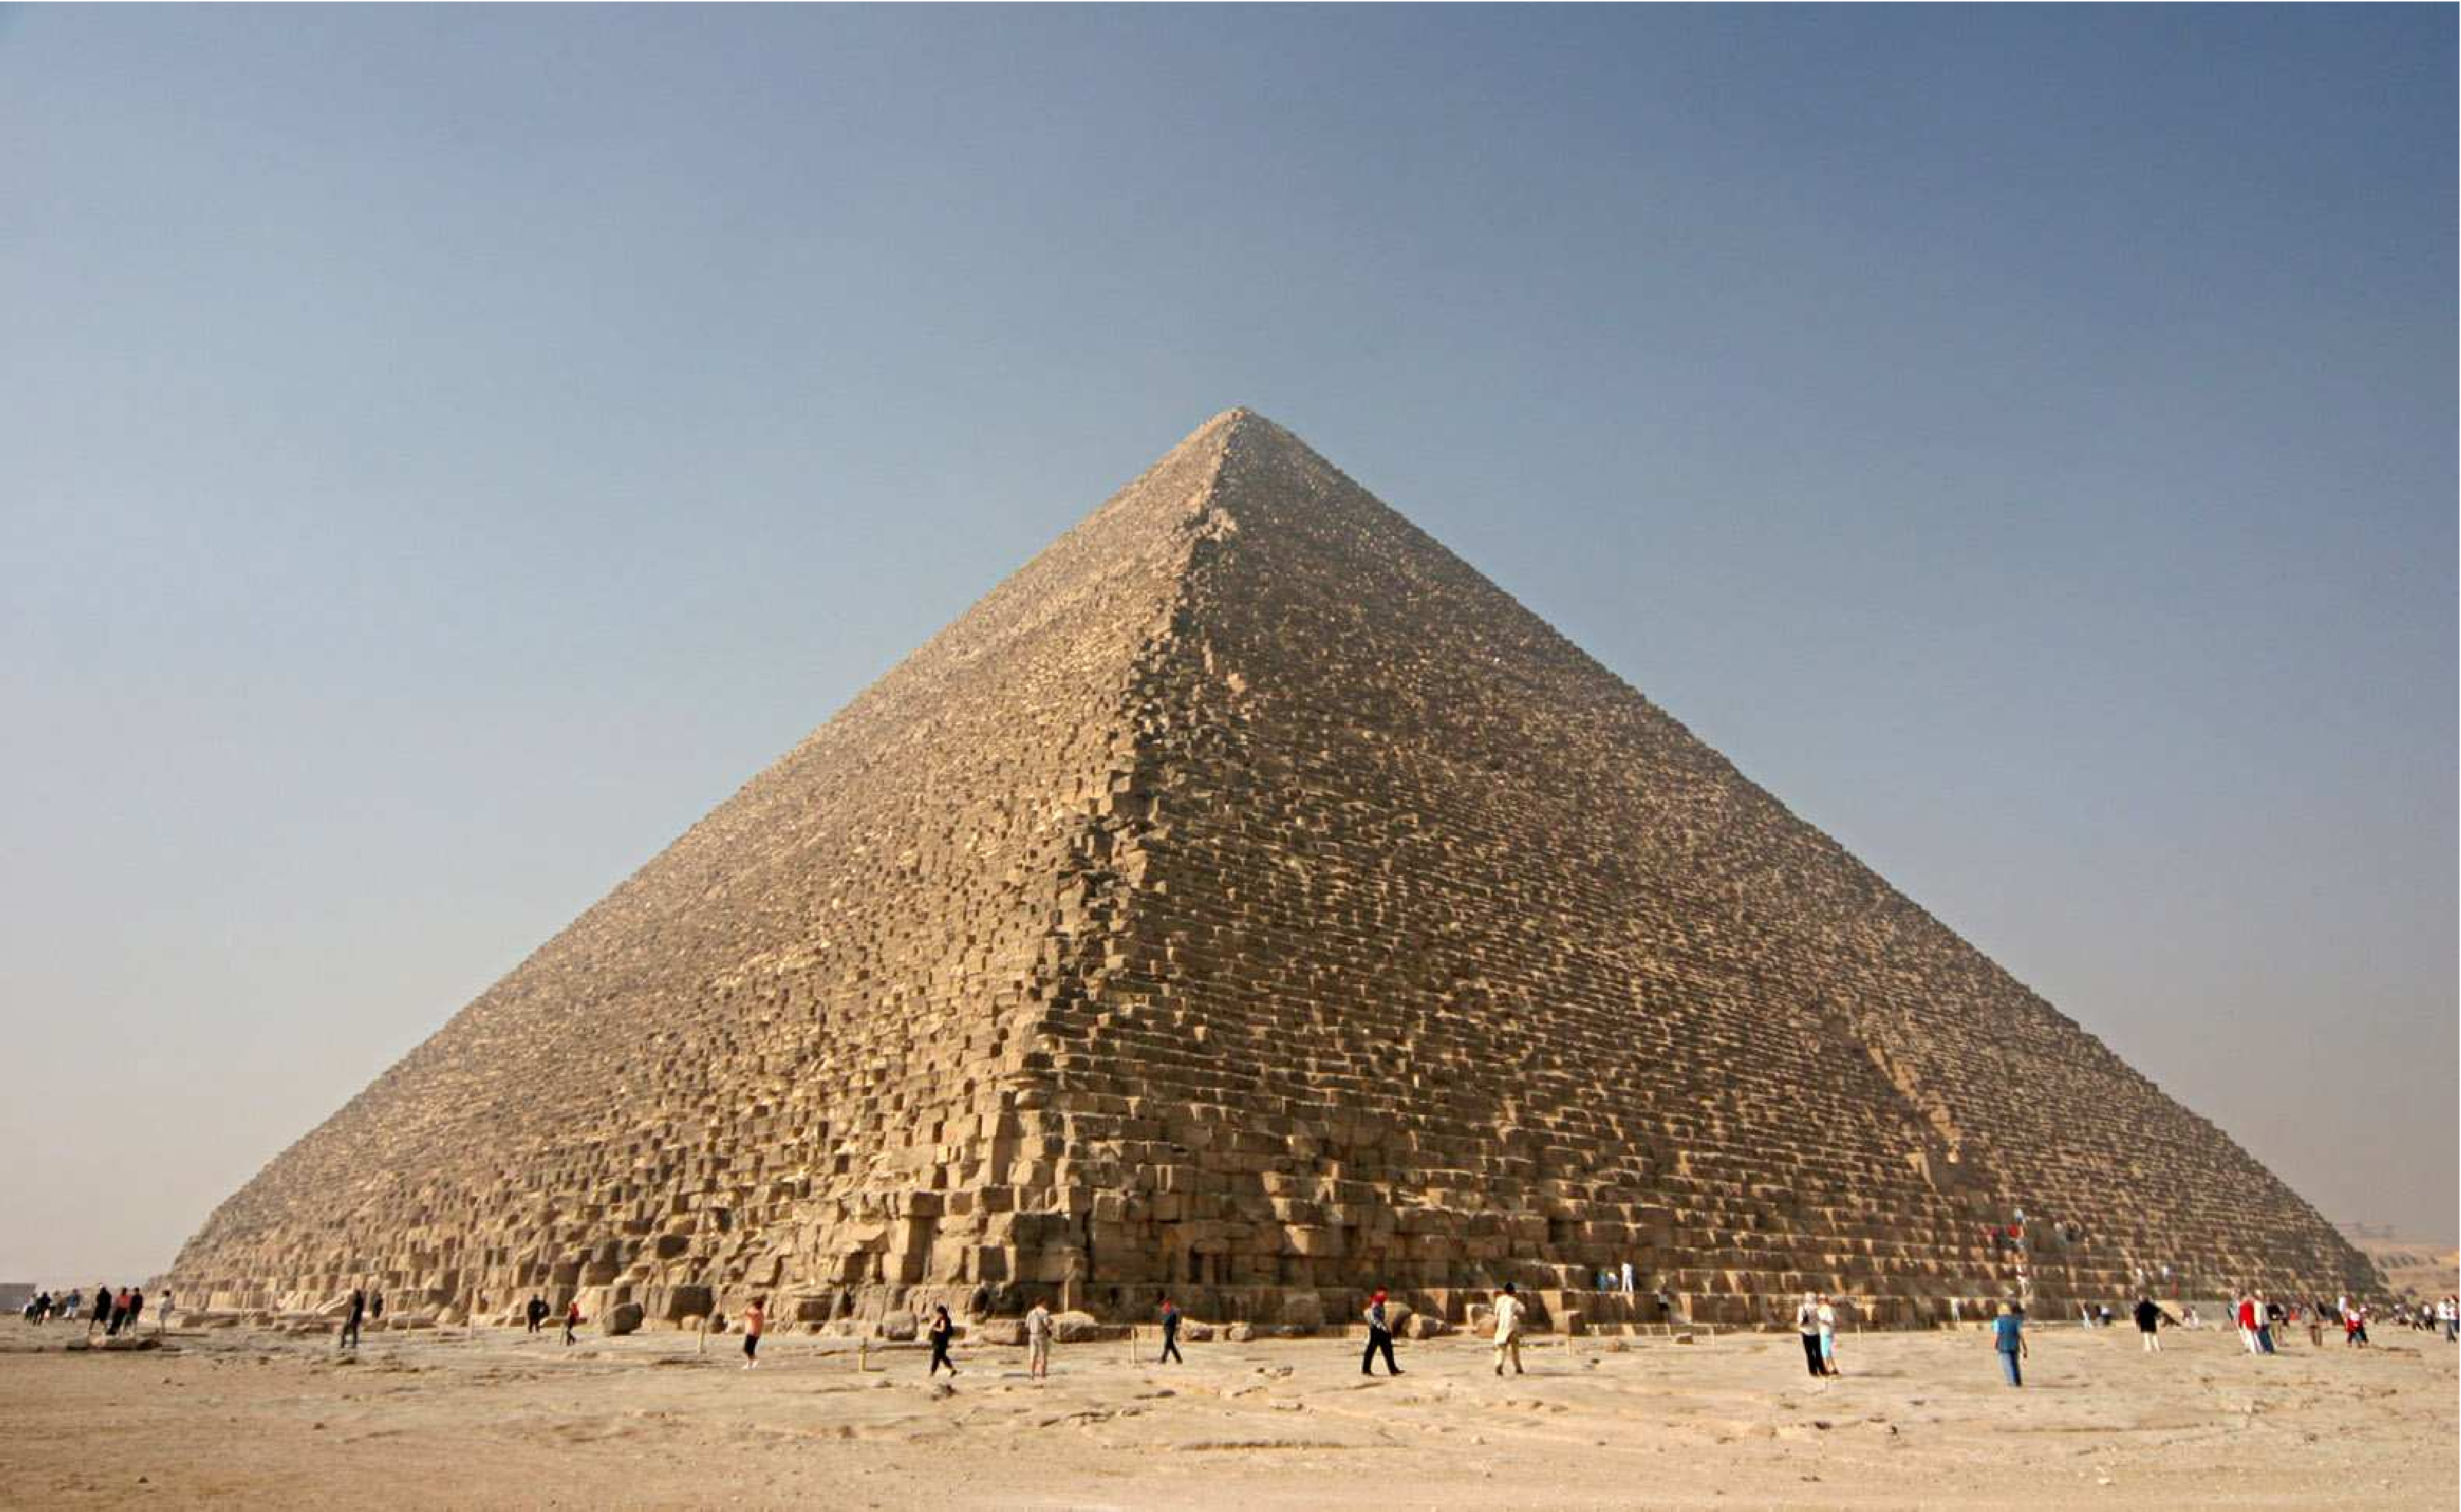
\includegraphics[height=0.8\textheight]{Fig/Kheops-Pyramid}
\end{center}
\end{frame}

\begin{frame}
\MadLogo
\frametitle{What is Science?}

\quotebox{{\Large \color{blue}{Science}} is the systematic enterprise
  of gathering knowledge about the universe and organizing and
  condensing that knowledge into testable laws and theories. The
  success and credibility of science are anchored in the willingness
  of scientists to {\color{red}{independent testing and replication}}
  by other scientists. This requires the  {\color{red}{complete and
      open exchange of data, procedures and materials}}.}{\\ American
  Physical Society}{What is Science?}

\end{frame}

\begin{frame}
\frametitle{From Science to Open-Source Software}

\quotebox{{\Large \color{blue}{Abandoning the habit of secrecy}} in favor of process
  transparency and peer review was the crucial step by which alchemy
  became chemistry.  In the same way, it is beginning to appear that
  open-source development may signal the long-awaited maturation of
  software development as a discipline.}  {\\ Eric Raymond}{TAUP,
  2004}
\end{frame}

\begin{frame}
\MadLogo
\frametitle{What is Reproducible Research?}

\begin{itemize}
\item Attaching software code and data to publications
\item Communicating computational results to a skeptic
\end{itemize}

\quotebox{An article about computational
    science in a scientific publication is not the scholarship itself,
    it is merely advertising of the scholarship. The actual
    scholarship is the complete software development environment and
    the complete set of instructions which generated the figures.}
  {Jon Buckheit and David Donoho}{WaveLab}

\end{frame}

\begin{frame}
 \frametitle{Reproducible Research Discussions}

\begin{itemize}
\item {\color{blue}{\textbf{\url{http://www.reproducibleresearch.net} }}}
\end{itemize}

  \begin{minipage}{0.3\textwidth}
  \begin{center}
  \framebox{
\includegraphics[width=\textwidth]{Fig/CiSE}}
  \vfill \ 
\end{center}
  \end{minipage} \hfill
   \begin{minipage}{0.65\textwidth}
  \begin{description}
    \item[ICASSP 2007] \ 
    \item[Berlin-6 2008] \
    \item[CiSE 2009] 
    \begin{itemize}
%    \item Fomel \& Claerbout
    \item Donoho et al.
    \item LeVeque
    \item Ping \& Eckel
    \item Stodden
    \end{itemize}
    \item[IEEE Signal Processing Magazine 2009] 
    \begin{itemize}
    \item Vandewalle et al.
     \end{itemize}
     \item[Yale Roundtable 2009] \
     \item[NSF Archive Workshop 2010] \ 
   \end{description}
  \end{minipage}
\end{frame}

\begin{frame}
  \MadLogo
  \frametitle{Jon Claerbout's Story}

  {\flushright
  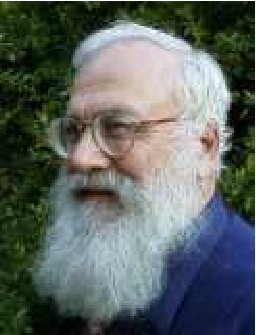
\includegraphics[height=0.2\textheight]{Fig/Claerbout}
  } 

  \begin{description}
  \item[1987] Sunview experience
  \begin{itemize}
  \item	Interactive programs are slavery
  \end{itemize}
  \item[1992] \LaTeX\ + \texttt{cake}
  \begin{itemize}
  \item Building books by a single command
  \end{itemize}
  \item[1990s] Ph.D. students
  \begin{itemize}
  \item \texttt{cake} to \texttt{make}, CD-Rom to WWW
  \end{itemize}
  \item[2001] Reproducible research paper in \emph{CiSE}
  \begin{itemize}
  \item {\color{blue}{The principal beneficiary is the author}}
  \end{itemize}
  \end{description}
\end{frame}

\begin{frame}
  \MadLogo
  \frametitle{Reproducibility Laws}
  \begin{itemize}
  \item The principal beneficiary is the author
  \item Software code requires continuous maintenance
  \item Maintenance requires an open community
  \end{itemize}
\end{frame}

\begin{frame}
  \begin{center}
 
\includegraphics[height=0.25\textheight]{Fig/MadLogo} \\
 {\color{blue}{\textbf{\url{http://ahay.org/}}}} 
  \end{center}
\end{frame}

\begin{frame}
  \frametitle{Basic Facts about \textsc{Madagascar}}
\bfseries
  \begin{itemize} 
  \item Publicly available since June 12, 2006 
  \item GPL licensed
  \item 1.0 version released on July 22, 2010
  \item 25+ developers
  \item 250,000+ lines of code
  \item 10,000+ downloads from {\color{blue}{\href{http://sourceforge.net/projects/rsf/}{SourceForge}}}
  \item
    {\color{blue}{\textbf{\url{http://www.ahay.org/wiki/Reproducible_Documents}}}}
\end{itemize}
\end{frame}

\begin{frame}
  \MadLogo
\begin{center}
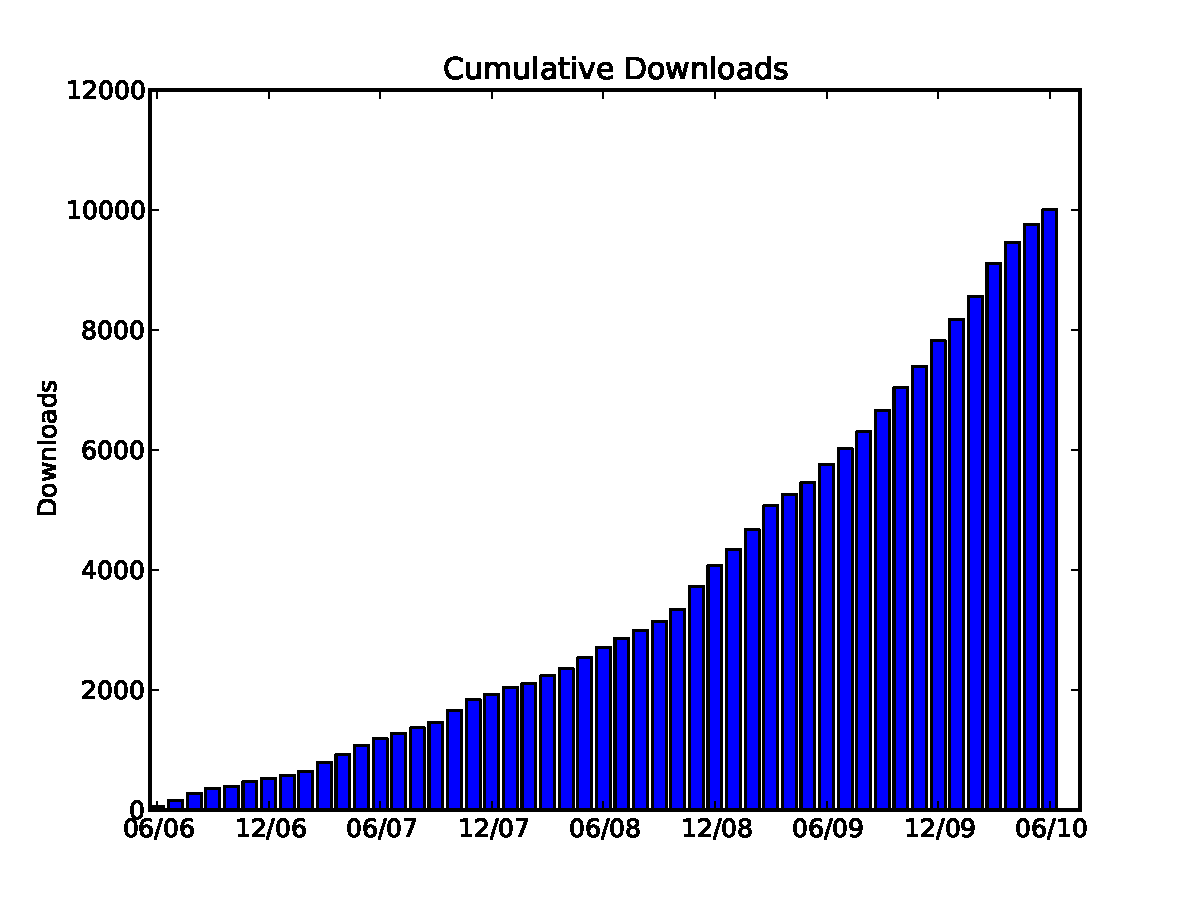
\includegraphics[height=\textheight]{Pylab/Fig/downloads}  
\end{center}
\end{frame}

\begin{frame}
  \MadLogo
  \frametitle{Access Geography}
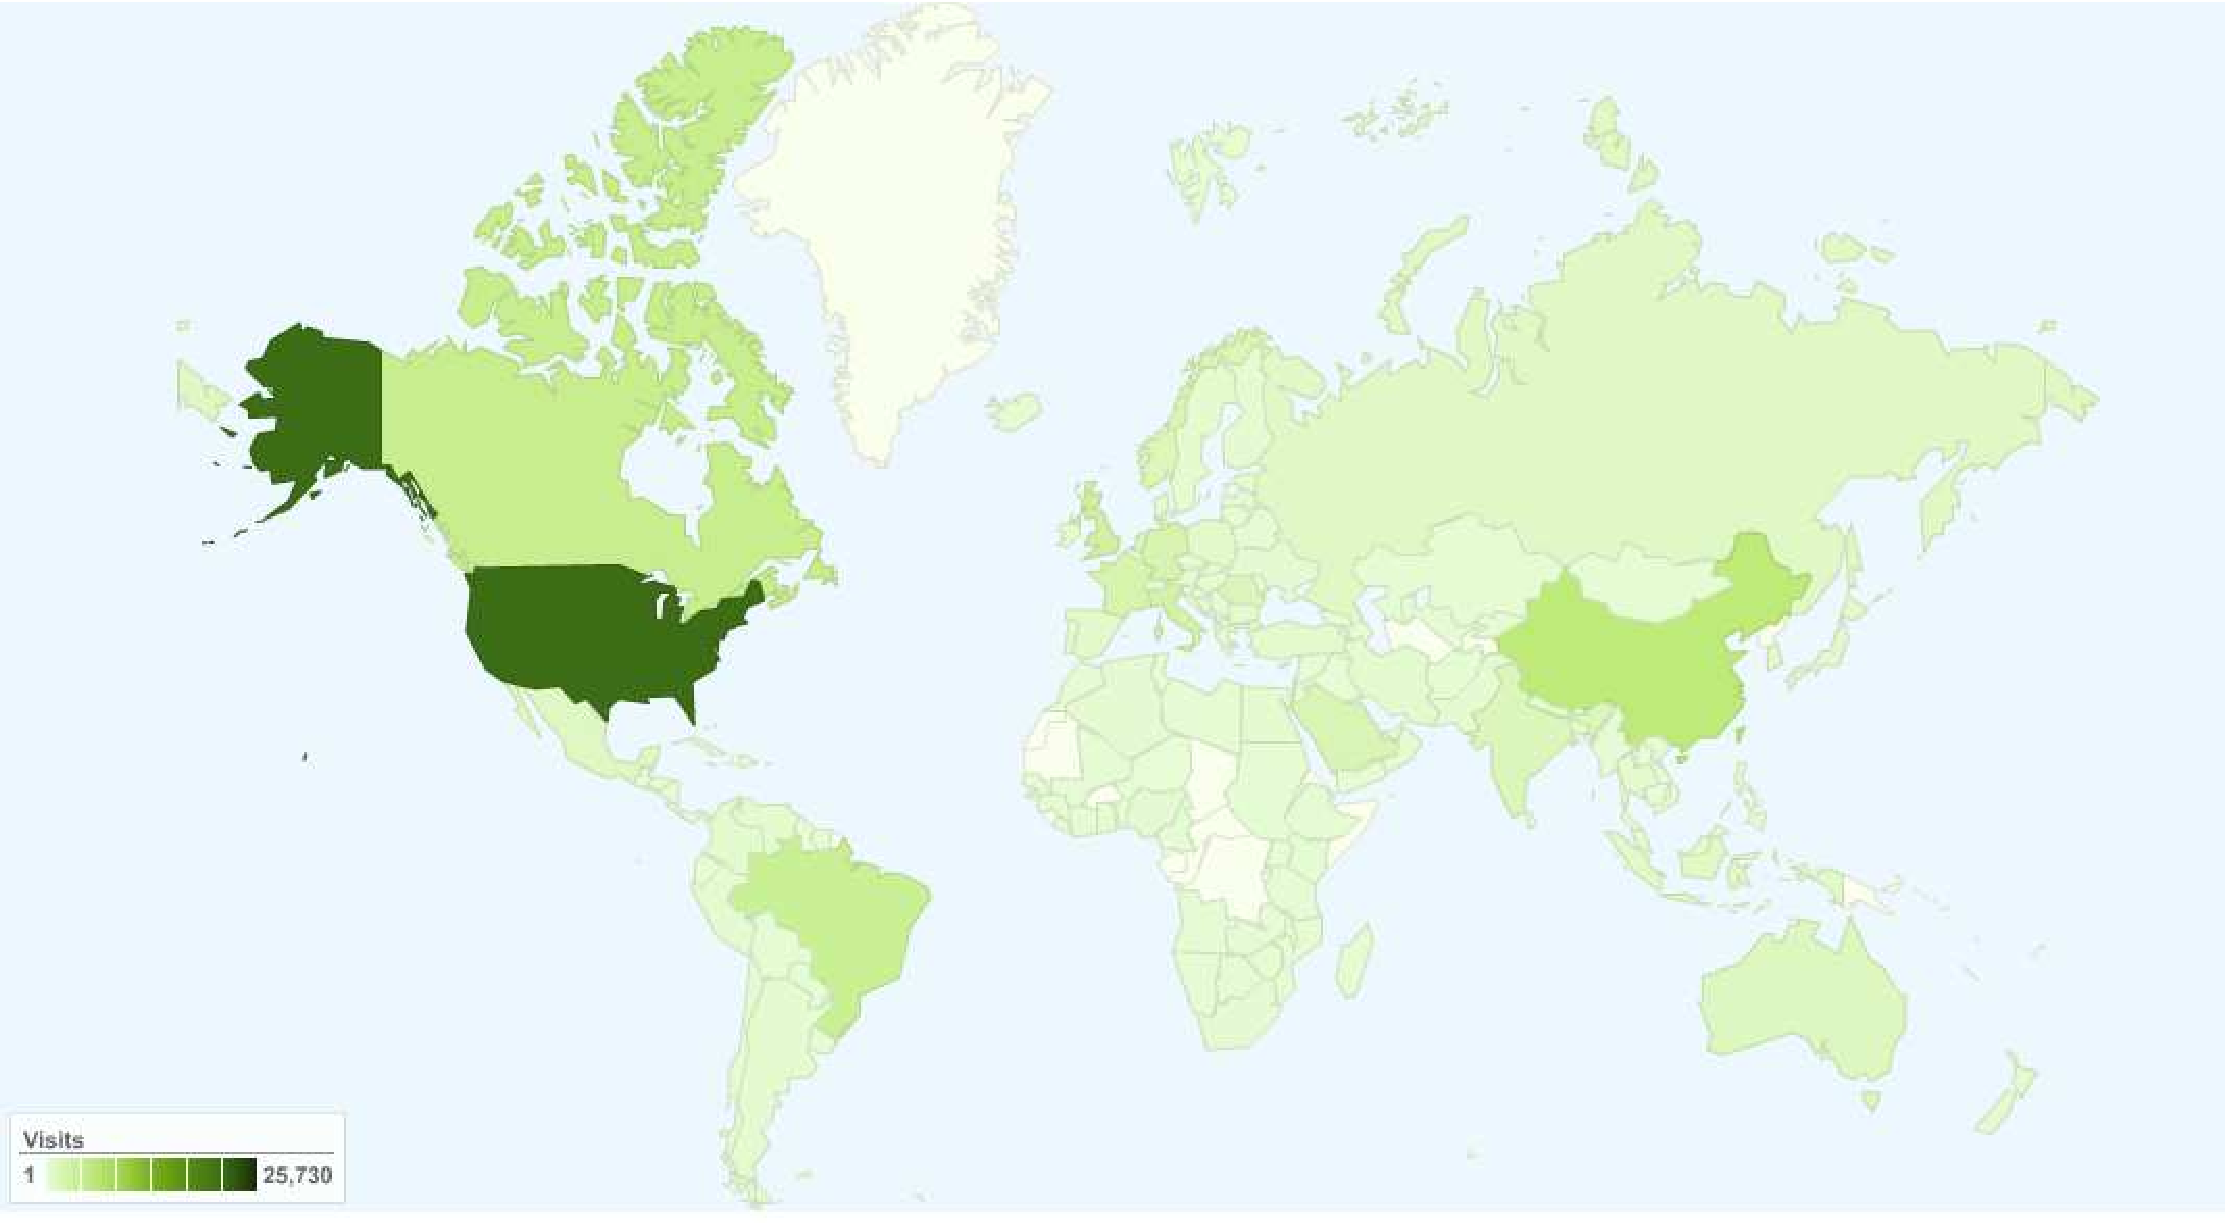
\includegraphics[width=\textwidth]{Fig/map}  
\end{frame}

\begin{frame}
  \frametitle{School and Workshop: Vancouver 2006}
  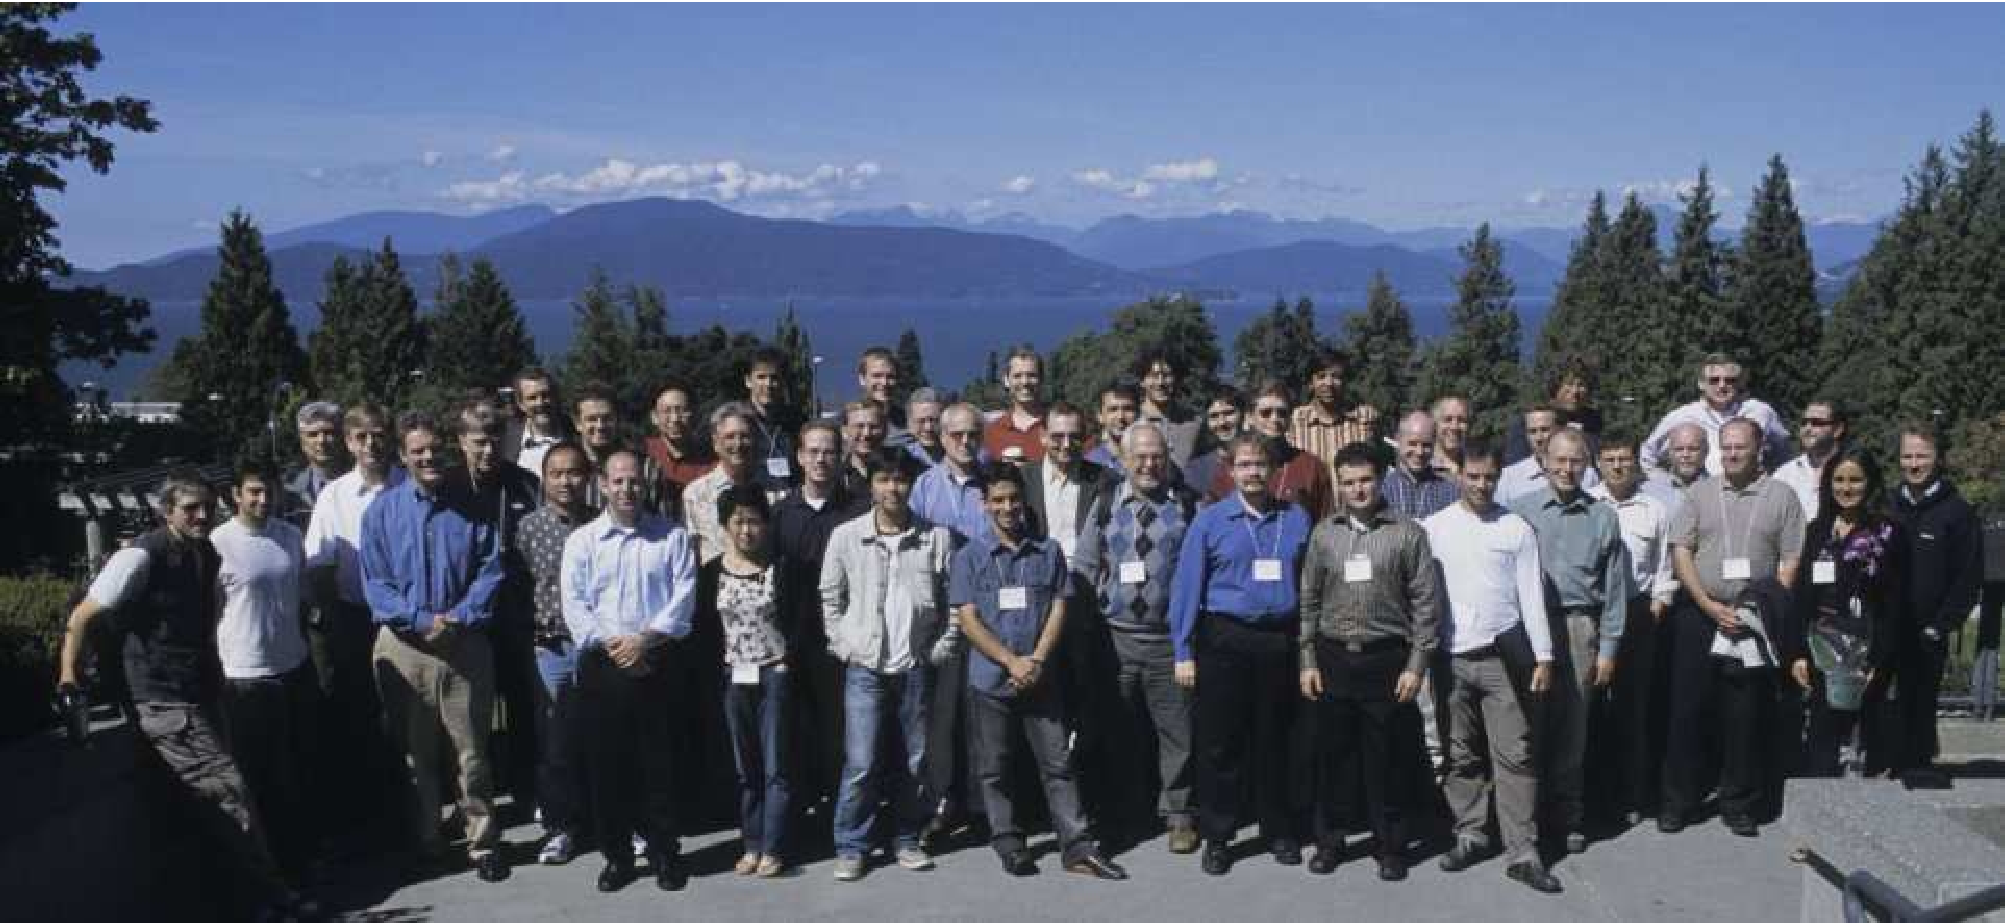
\includegraphics[width=\textwidth]{Fig/RSF2006}
\end{frame}

\begin{frame}
  \frametitle{School: Austin 2007}
  \begin{minipage}{0.45\textwidth} 
  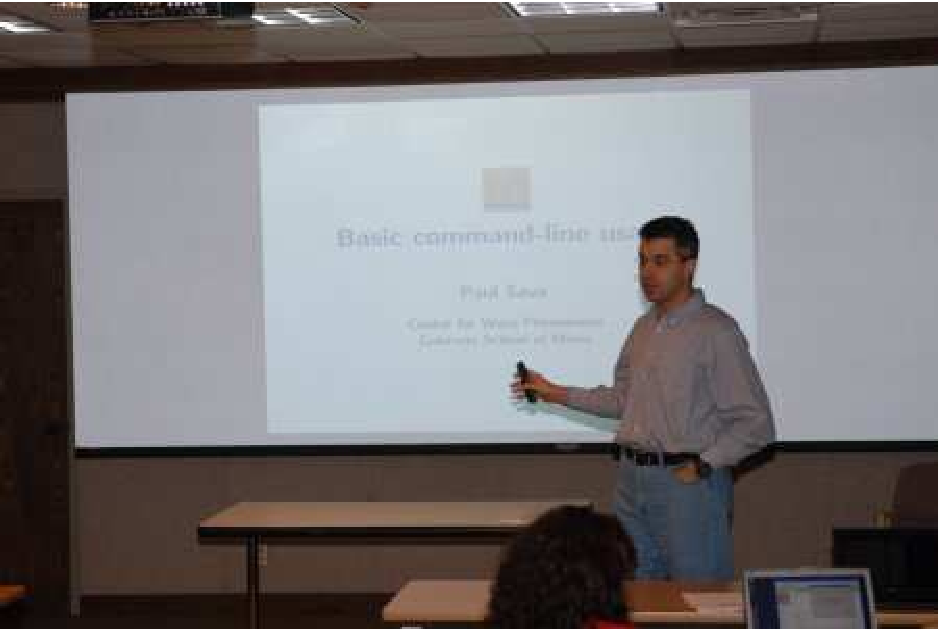
\includegraphics[width=\textwidth]{Fig/Paul}
   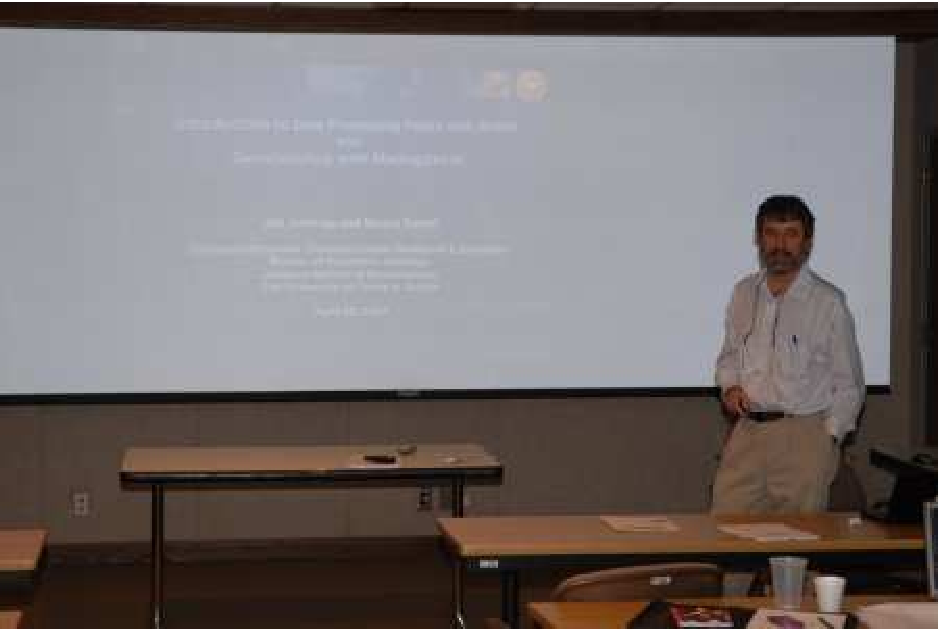
\includegraphics[width=\textwidth]{Fig/Jim}
  \end{minipage} \hfill
  \begin{minipage}{0.45\textwidth}
  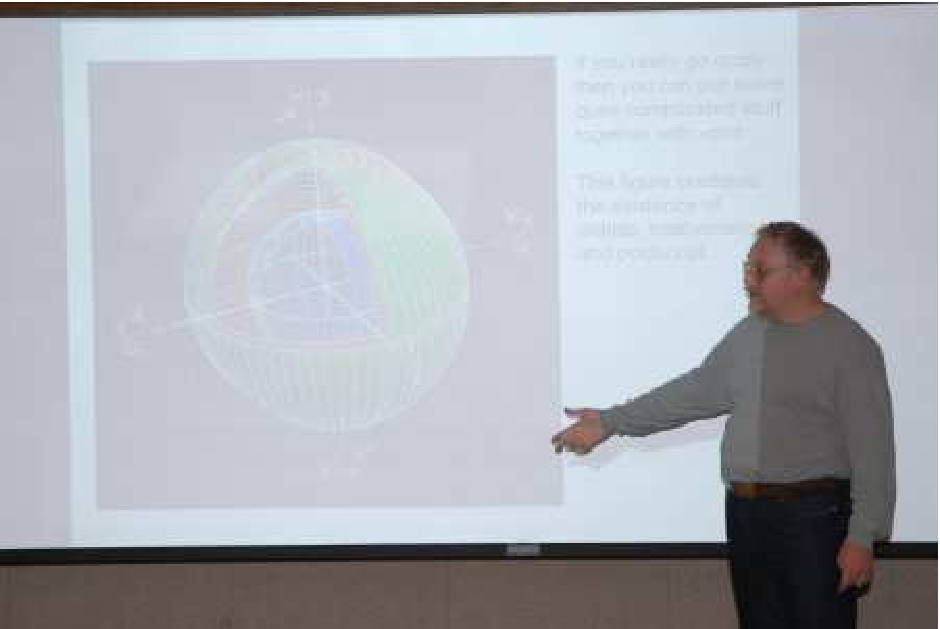
\includegraphics[width=\textwidth]{Fig/Joe}
   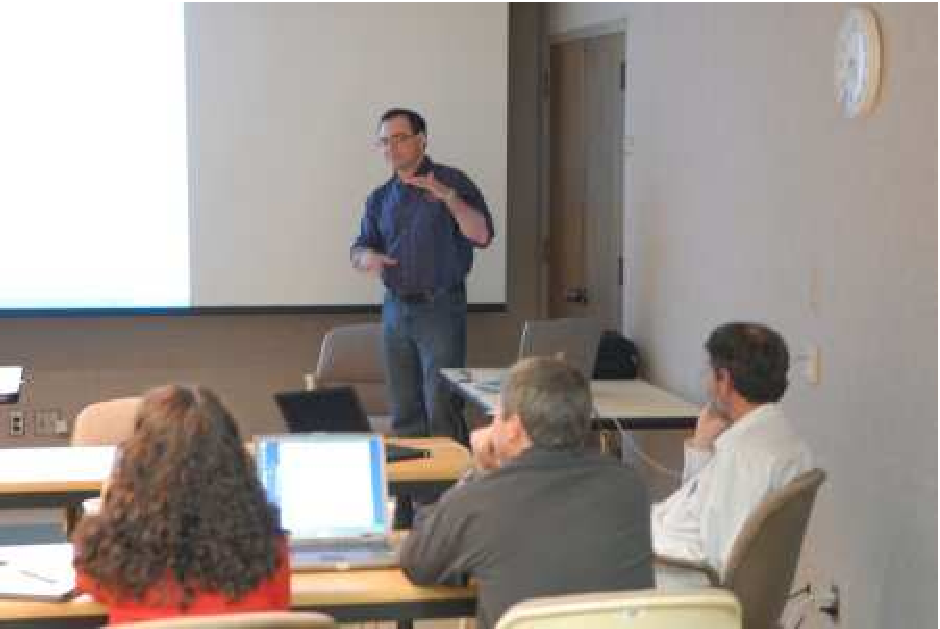
\includegraphics[width=\textwidth]{Fig/Sergey}
   \end{minipage}
\end{frame}

\begin{frame}
  \frametitle{Developer Workshop: Golden 2008}
  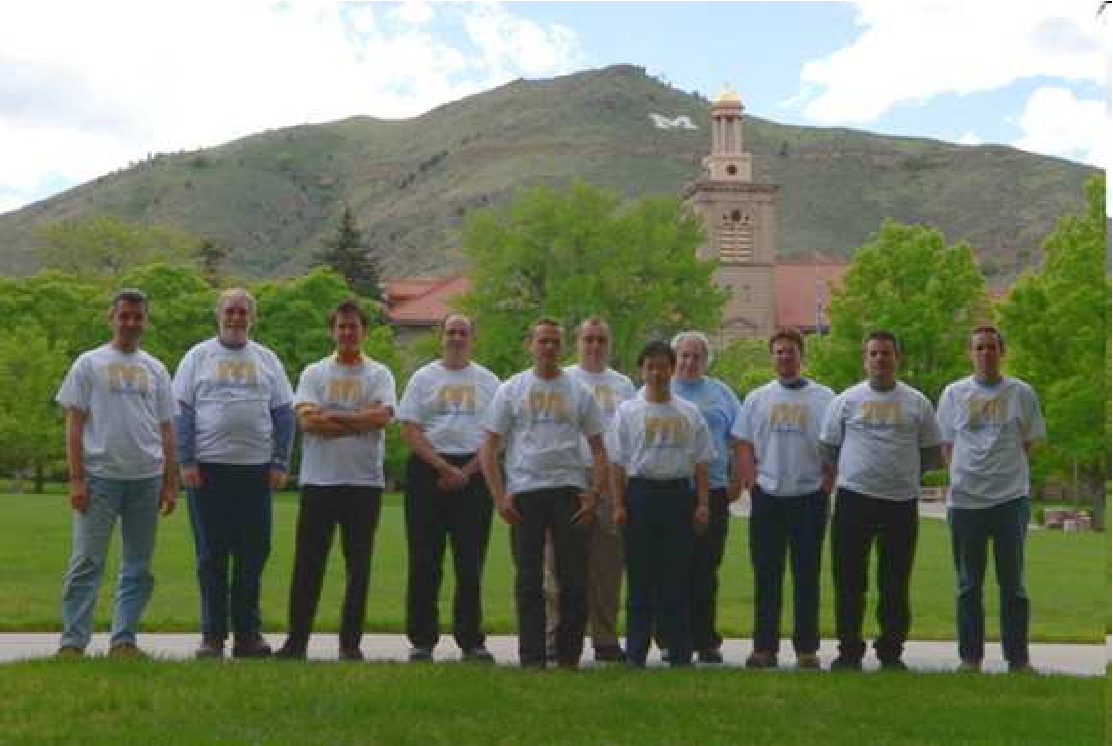
\includegraphics[height=0.7\textheight]{Fig/RSF2008}
\end{frame}

\begin{frame}
  \frametitle{School and  Workshop: Delft 2009}
  \begin{itemize}
  \item More than 50 people
  \item 30 organizations (20 universities and 10  companies) 
  \item 15 countries  
  \end{itemize}
\end{frame}

\section{\textsc{Madagascar} Components}

\begin{frame}<beamer>
  \MadLogo
  \frametitle{Outline}
  \tableofcontents[currentsection]
\end{frame}

\begin{frame}
  \MadLogo
  \frametitle{Obtaining \textsc{Madagascar}}
  \begin{itemize}
    \item Download stable release from
      {\color{blue}{\href{http://sourceforge.net/projects/rsf/}{SourceForge}}}
    \item Use \texttt{svn} (Subversion) to download {\color{blue}{\href{http://sourceforge.net/p/rsf/code/HEAD/tree/trunk/}{unstable}}} (current
      development) release
      \begin{itemize}
        \item \texttt{svn checkout}
        \item \texttt{svn update}
        \item \texttt{svn commit} (developers)
      \end{itemize}
  \end{itemize}
\end{frame}

\begin{frame}
  \frametitle{Installing \textsc{Madagascar} from Source}
  \begin{itemize}
  \item \texttt{./configure --prefix=/directory/name}
  \item \texttt{make}
  \item \texttt{make install}
  \end{itemize}
  \begin{center}
  Full details at
  {\color{blue}{\url{http://www.ahay.org/wiki/Installation}}} \\
  {\color{blue}{\url{http://www.ahay.org/wiki/Advanced_Installation}}}
\end{center}
\end{frame}

\begin{frame}
  \MadLogo

  \frametitle{One Week Technology Transfer}
  \begin{tabular}{rl}
  \textbf{\color{blue}{Monday:}} & Get an idea \\
  \textbf{\color{blue}{Tuesday:}} & Implement it \\
  \textbf{\color{blue}{Wednesday:}} & Test it \\
  \textbf{\color{blue}{Thursday:}} & Communicate it \\
  \textbf{\color{blue}{Friday:}} & Apply it in practice
  \end{tabular}
\end{frame}

\begin{frame}
  \MadLogo
  \frametitle{\textsc{Madagascar} Components}

    \begin{description}
    \item[Tuesday:] Implement it
      \begin{itemize}
      \item Main programs (C, C++, Fortran, Python, etc)
      \item \href{http://www.reproducibility.org/RSF/}{750 modules}
      \end{itemize}
    \item[Wednesday:] Test it
      \begin{itemize}
      \item Data processing flows (Python/SCons)
      \item 350 scripts $\rightarrow$ 3,200 figures
      \end{itemize}
    \item[Thursday:] Communicate it
      \begin{itemize}
      \item Books and papers (\LaTeX/SCons)
      \item \href{http://www.ahay.org/Reproducible_Documents}{100 papers}
      \end{itemize}
    \end{description}
\end{frame}

\begin{frame}
  \MadLogo
  \frametitle{\textsc{Madagascar} Objectives}

  \begin{itemize}
  \item To make computational research efficient
  \item To make it easy to share computational results
  \item To promote an open community
  \end{itemize}
\end{frame}

\begin{frame}
  \MadLogo
  \frametitle{\textsc{Madagascar} Design Principles}

  \begin{itemize}
  \item Document computational experiments and use them in the future as regression {\color{blue}{tests}}
  \item {\color{blue}{Reproducible research}}
  \item YAGNI (You Ain't Gonna Need It)
  \item Encapsulation and modularity
  \end{itemize}
  \quotebox{Always implement things when you actually need them, never
    when you just foresee that you need them.}{Ron Jeffries}{YAGNI}  
  \quotebox{Write programs that do one thing and do it well. Write
        programs to work together. Write programs to handle text
        streams, because that is a universal interface.}{Doug McIlroy}{Unix}
\end{frame}

\begin{frame}
  \MadLogo
  \frametitle{RSF File Format}

\begin{minipage}{0.3\textwidth}
  \begin{center}
  \framebox{
\includegraphics[width=\textwidth]{Fig/unix}}
  \vfill \ 
\end{center}
  \end{minipage} \hfill
   \begin{minipage}{0.65\textwidth}
\begin{itemize}
  \item Multidimensional arrays as files
  \item Simple universal \href{http://www.ahay.org/Format}{data file format}
  \begin{itemize}
  \item mostly compatible with SEPlib
  \end{itemize}
  \item Data separated from text headers
  \item Conceptually $N$-D hypercubes
  \item Multiple files for irregular data
  \end{itemize}
\quotebox{If you feel an urge to design a complex binary file format,
  or a complex binary application protocol,  it is generally wise to lie down until the feeling passes.}{Eric Raymond}{TAUP}
  \end{minipage}
  
\end{frame}

\begin{frame}
\frametitle{\textsc{Madagascar} filter in C}
\MadLogo

\begin{code}[c]
\centering
\hfill
\begin{minipage}{0.9\textwidth}
\lstset{language=c,showstringspaces=false}
\lstinputlisting[frame=single]{clip.c}
\end{minipage}
\hfill
\end{code}

\end{frame}

\begin{frame}
\frametitle{\textsc{Madagascar} filter in Python}
\MadLogo

\begin{code}[python]
\centering
\hfill
\begin{minipage}{0.9\textwidth}
\lstinputlisting[frame=single]{clip.py}
\end{minipage}
\hfill
\end{code}

\end{frame}

\begin{frame}
\frametitle{\textsc{Madagascar} \texttt{SConstruct} script}
\MadLogo

\begin{code}[python]
\centering
\hfill
\begin{minipage}{0.9\textwidth}
\lstinputlisting[frame=single]{scons.py}
\end{minipage}
\hfill
\end{code}

\vfill

\begin{code}[bash]
\lstinputlisting[frame=none]{scons.sh}
\end{code}

\vfill
\begin{itemize}
\item  {\color{blue}{\textbf{\url{http://www.scons.org/}}}}
\end{itemize}
\end{frame}

\begin{frame}
\MadLogo
\frametitle{Goal for \textsc{Madagascar} 1.0}
\begin{itemize}
\item Automatic Testing
\end{itemize}
\end{frame}

\begin{frame}
\MadLogo
\frametitle{Goals for \textsc{Madagascar} 2.0}
\begin{itemize}
\item High-performance computing
\item Seismic field data processing examples
\item Applications beyond seismic
\end{itemize}
\end{frame}

\begin{frame}
\MadLogo
\frametitle{Conclusions}
\bfseries
\centering
  \begin{itemize}
  \item Reproducible research
    \begin{itemize}
    \item Attaching software and data to publications
    \item Computational experiments communicated to a skeptic
    \item Continuous maintenance requires an open community
    \end{itemize}
  \item \textsc{Madagascar} Objectives
    \begin{itemize}
    \item To make computational research efficient
    \item To make it easy to share computational results
    \item To promote an open community
    \end{itemize}
\end{itemize}
    \begin{center}
      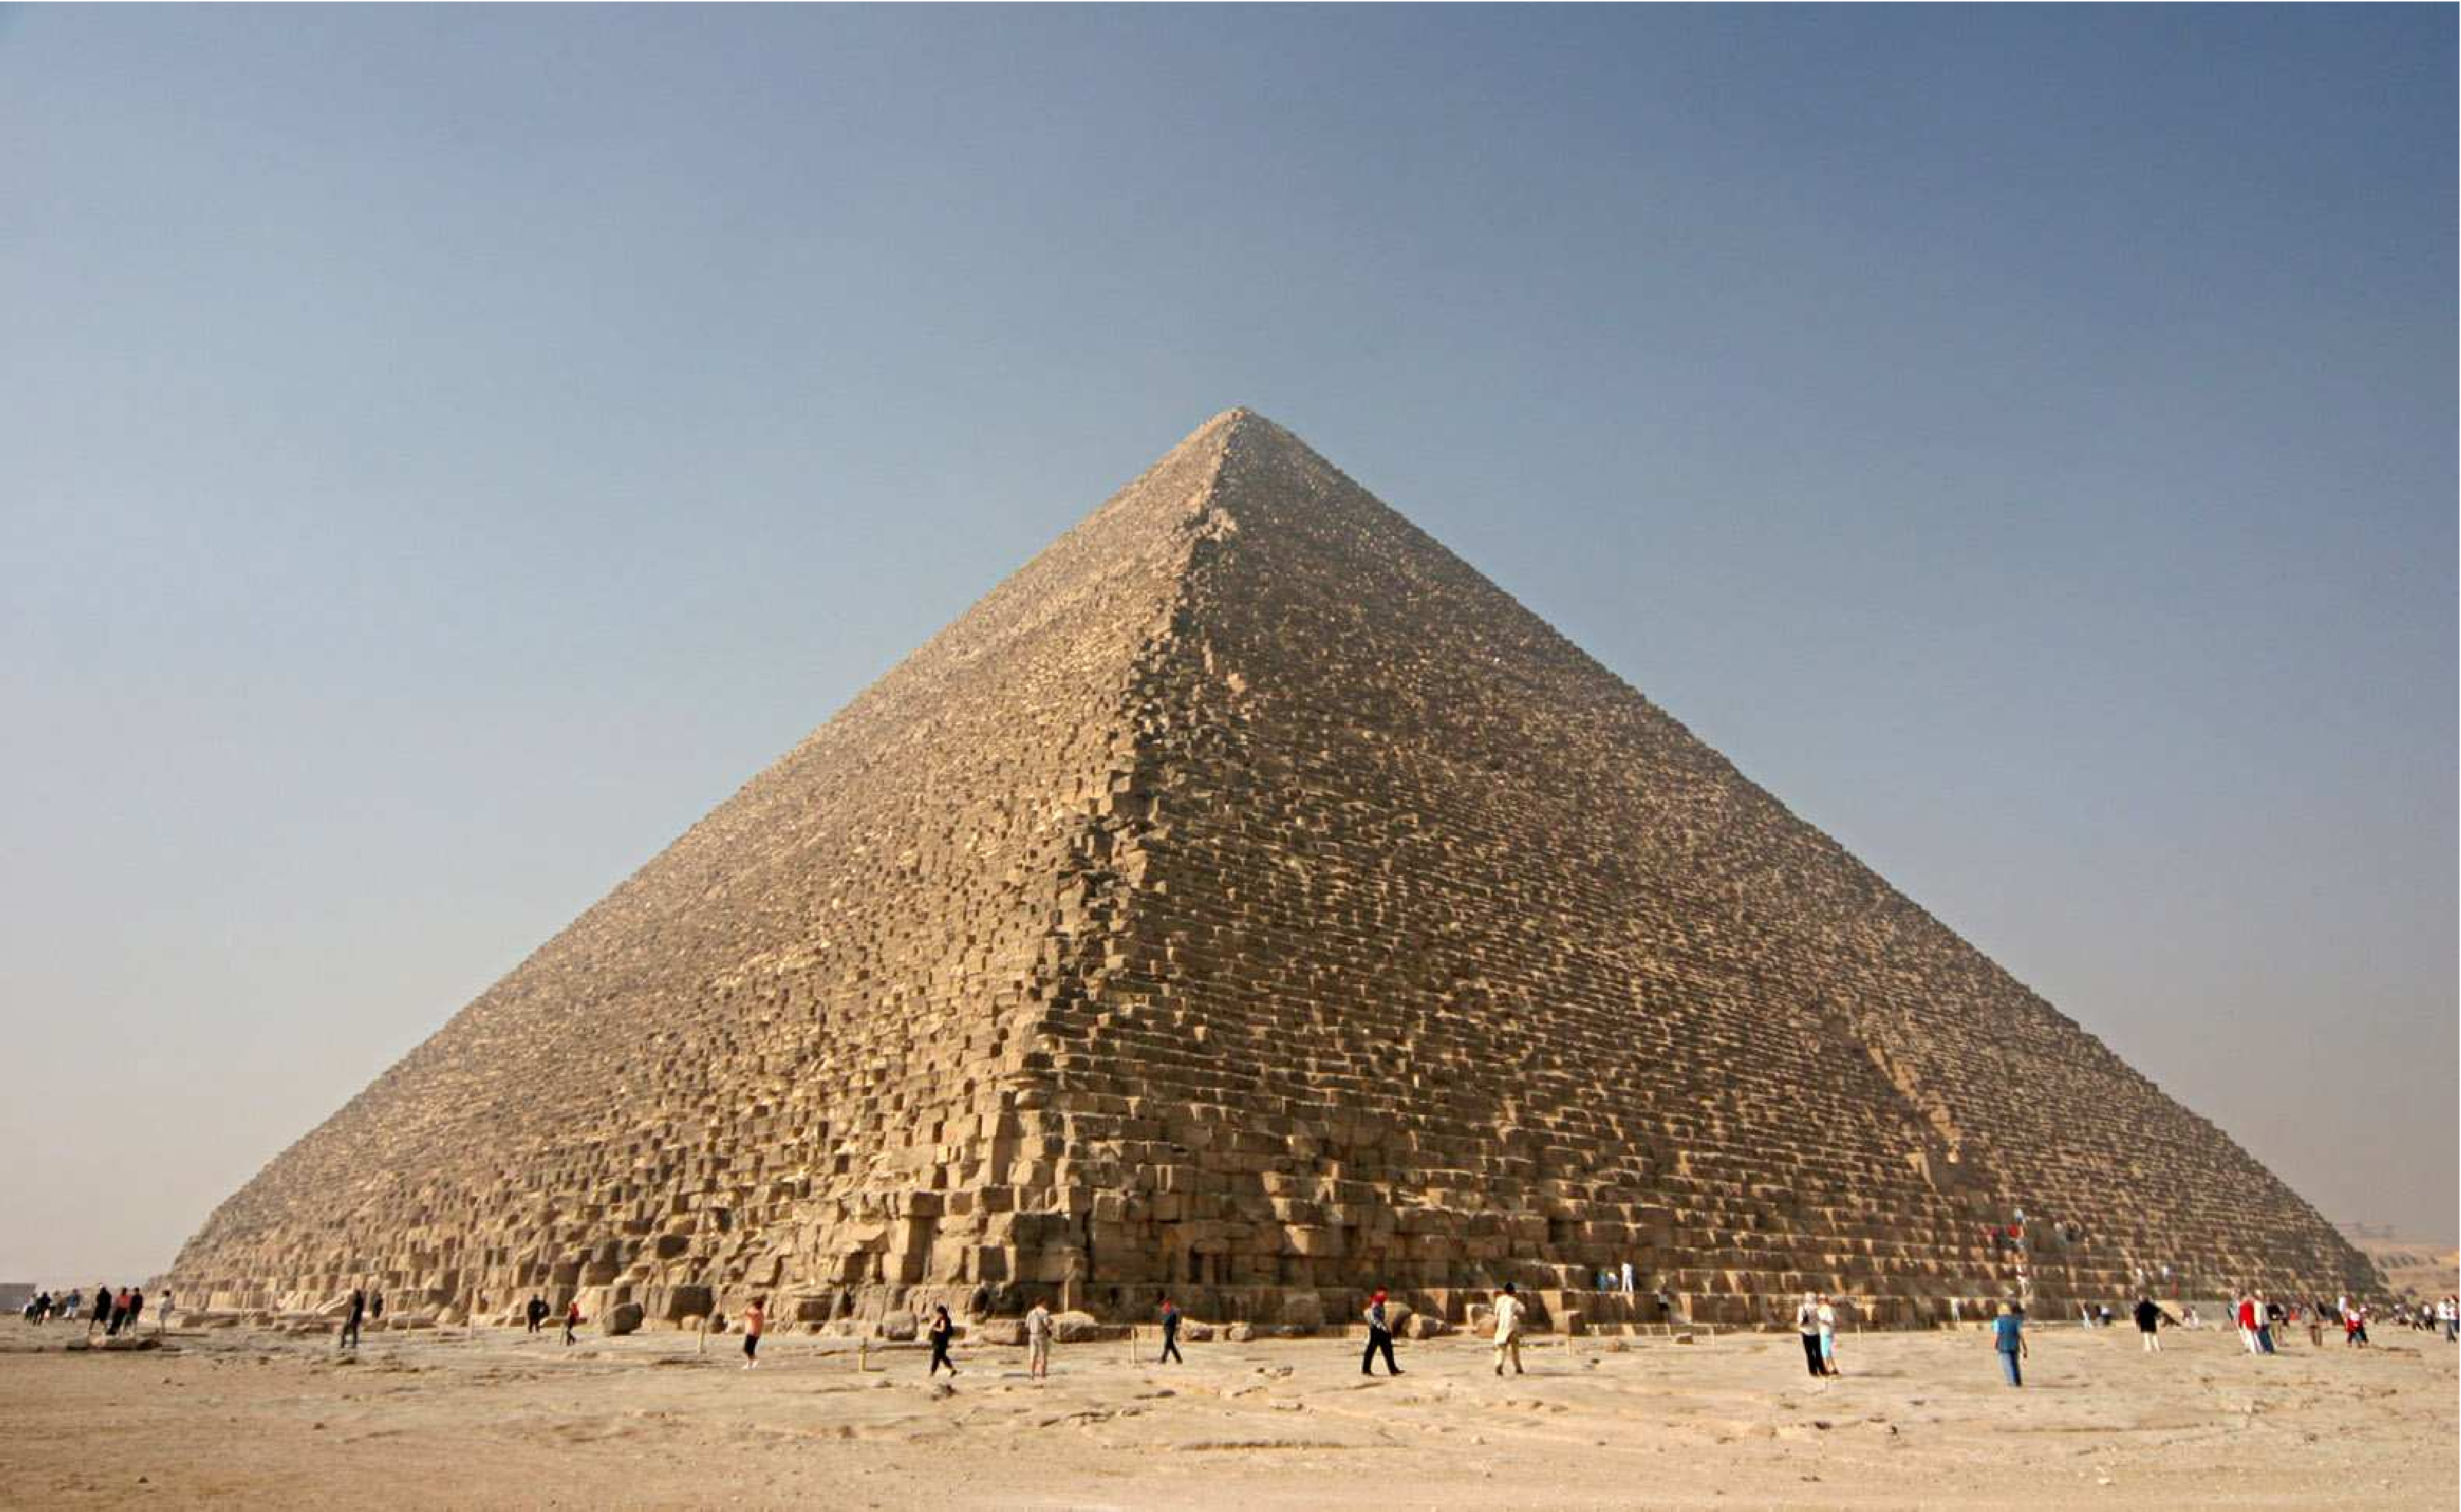
\includegraphics[height=0.4\textheight]{Fig/Kheops-Pyramid}
    \end{center}
  \end{frame}
